\chapter{Babylon Falls, and the Lamb Is Victorious (17:1--18:24)}\index{Babylon}\index{Lamb, the}

Babylon\index{Babylon} represents a world system that seduces humanity through luxury, power, and economic gain.

John sees a woman clothed in splendor, seated upon a scarlet beast. Gold, precious stones, and pearls adorn her. She has joined herself to the kings of the earth, intoxicated the nations, and enriched the merchants of the world through her extravagant wealth. Yet beneath her dazzling appearance lie corruption, idolatry, immorality, pride, and the persecution\index{persecution} of God's people. She appears powerful, prosperous, and unshakable. But God declares that her fall is certain.

The greatest danger Babylon\index{Babylon} poses is not simply her open hostility toward God, but her irresistible allure. Through wealth, success, influence, luxury, and pleasure, she persuades the world that these things constitute the glory\index{glory} for which life is meant. She does not always demand that people deny God outright. More often, she quietly teaches them to place their security in riches, measure their worth by success, entrust their hopes to power, and seek fulfillment in material abundance.

The message of Babylon\index{Babylon}, therefore, is not reserved for readers contemplating the end of the age. It speaks to every Christian who lives in the world today.

Our work, our businesses, our use of money and technology, and the resources available to us in society can all be good gifts from God. Nor can we withdraw entirely from the world in which He has placed us. The question is not whether we use these things, but whether we begin to worship\index{worship} them; not whether we possess wealth, but whether wealth has begun to possess our hearts. God does not call His people to flee the world altogether. He calls them to resist being conformed to its values.

That is why God issues His people a clear and urgent command:

“My people, come out of her, so that you will not share in her sins.” (Revelation 18:4, NIV)

Revelation places two women before our eyes: Babylon\index{Babylon}, seated upon the beast\index{beast}, and the Church, making herself ready for the Lamb\index{Lamb, the}. One embodies the splendor of the earth; the other, the glory of heaven. One appears invincible but falls in an instant; the other may seem weak in the eyes of the world, yet belongs forever to the victorious Lamb.

May we remain faithful to Christ in the midst of this world, preserving holiness amid temptation, keeping our spiritual vision clear amid material allurements, and worshiping the true King of kings\index{King of kings} even when earthly powers demand our allegiance.

\section{Babylon}\index{Babylon}

\begin{ScriptureBox2}{Circle every detail of the woman's clothing and what she holds. What is written on her forehead, and what is she drunk with?}

\item[17:1] One of the seven angels who had the seven bowls came and said to me, ``Come, I will show you the punishment of the great prostitute, who sits by many waters.

\item[17:2] With her the kings of the earth committed adultery, and the inhabitants of the earth were intoxicated with the wine of her adulteries.''

\item[17:3] Then the angel carried me away in the Spirit into a wilderness. There I saw a woman sitting on a scarlet beast that was covered with blasphemous names and had seven heads and ten horns.

\item[17:4] The woman was dressed in purple and scarlet, and was glittering with gold, precious stones and pearls. She held a golden cup in her hand, filled with abominable things and the filth of her adulteries.

\item[17:5] The name written on her forehead was a mystery:\\
\hspace*{1em}\textsc{Babylon the Great}\\
\hspace*{1em}\textsc{the mother of prostitutes}\\
\hspace*{1em}\textsc{and of the abominations of the earth.}

\item[17:6] I saw that the woman was drunk with the blood of God's holy people, the blood of those who bore testimony to Jesus.\\
When I saw her, I was greatly astonished.

\item[17:7] Then the angel said to me: ``Why are you astonished? I will explain to you the mystery of the woman and of the beast she rides, which has the seven heads and ten horns.

\item[17:8] The beast, which you saw, once was, now is not, and yet will come up out of the Abyss and go to its destruction. The inhabitants of the earth whose names have not been written in the book of life from the creation of the world will be astonished when they see the beast, because it once was, now is not, and yet will come.

\end{ScriptureBox2}

\begin{figure}[htbp]
    \centering
    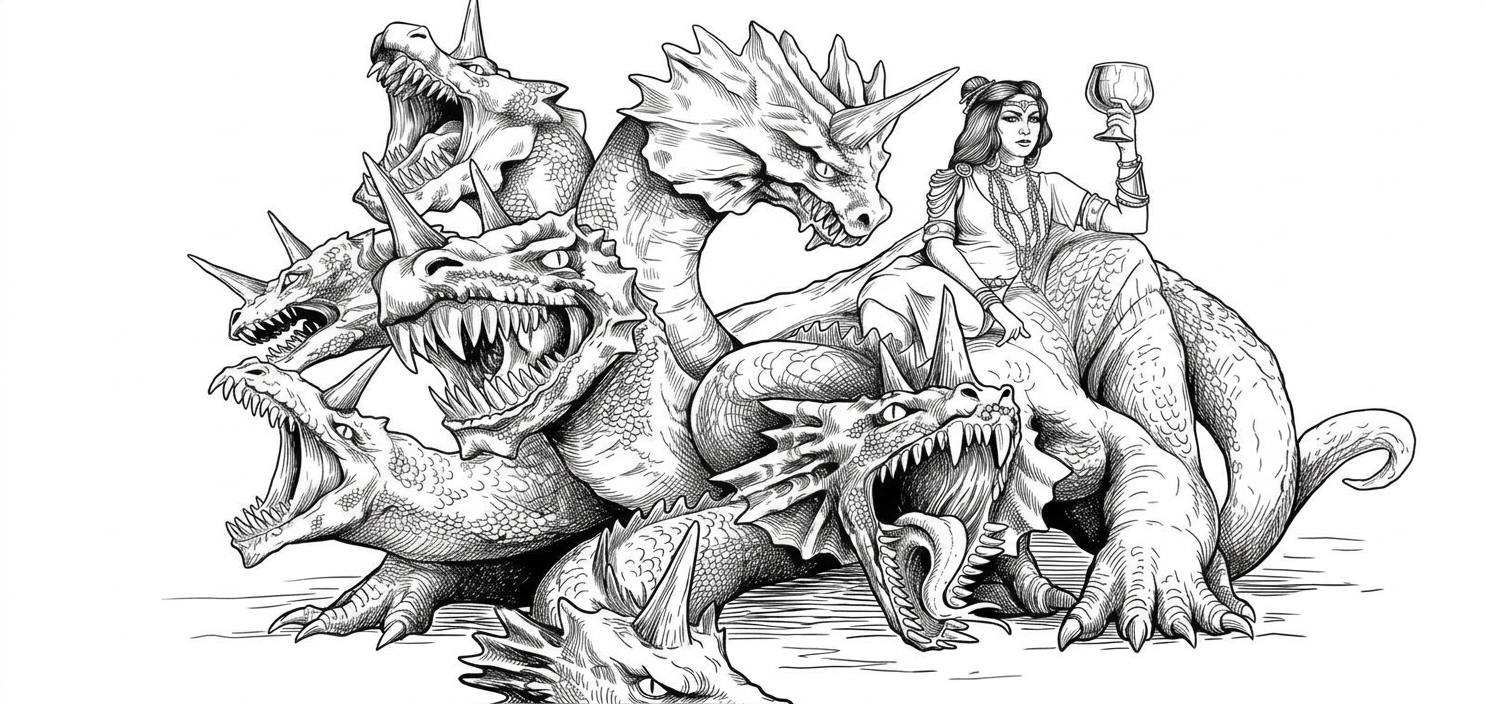
\includegraphics[
    width=1\textwidth,
    trim=0 0 0 0,
    clip]{images/babylon_harlot.jpg}
    %\caption{}
    %\label{}
\end{figure}

\begin{ScriptureBox2}{What do the seven heads, the ten horns, and the waters stand for? Underline who will triumph in 17:14, and why.}

\item[17:9] ``This calls for a mind with wisdom. The seven heads are seven hills on which the woman sits.

\item[17:10] They are also seven kings. Five have fallen, one is, the other has not yet come; but when he does come, he must remain for only a little while.

\item[17:11] The beast who once was, and now is not, is an eighth king. He belongs to the seven and is going to his destruction.

\item[17:12] ``The ten horns you saw are ten kings who have not yet received a kingdom, but who for one hour will receive authority as kings along with the beast.

\item[17:13] They have one purpose and will give their power and authority to the beast.

\item[17:14] They will wage war against the Lamb, but the Lamb will triumph over them because he is Lord of lords and King of kings---and with him will be his called, chosen and faithful followers.''

\item[17:15] Then the angel said to me, ``The waters you saw, where the prostitute sits, are peoples, multitudes, nations and languages.

\item[17:16] The beast and the ten horns you saw will hate the prostitute. They will bring her to ruin and leave her naked; they will eat her flesh and burn her with fire.

\item[17:17] For God has put it into their hearts to accomplish his purpose by agreeing to hand over to the beast their royal authority, until God's words are fulfilled.

\item[17:18] The woman you saw is the great city that rules over the kings of the earth.''

\end{ScriptureBox2}

“Babylon\index{Babylon}” may be understood as Rome\index{Rome} in the first century, or more broadly as the world system that sets itself against God. Accordingly, interpreters throughout the centuries have offered different explanations of the identities of Babylon and the ten kings.

The following table summarizes several major interpretations of the ten kings:

{
\renewcommand{\arraystretch}{1}
\small
\begin{longtable}{>{\raggedright\arraybackslash}p{3.6cm}
                  >{\raggedright\arraybackslash}p{5.4cm}}
\caption{Interpretations of the ten kings (Revelation 17)}
\label{tab:ten-kings} \\
\hline
Interpretation of the Ten Kings & Principal Basis \\
\hline
\endfirsthead

\multicolumn{2}{l}{\small\itshape Table~\thetable\ (continued)} \\
\hline
Interpretation of the Ten Kings & Principal Basis \\
\hline
\endhead

\hline
\endfoot

\hline
\endlastfoot

An alliance of ten political powers at the end of the age &
Revelation 17:12--13, which describes ten kings who receive authority with the beast for a brief time. \\

Ten emperors in the history of first-century Rome &
Revelation 17:10: ``Five have fallen, one is, the other has not yet come.'' \\

Empires drawn from the visions of Daniel &
Emphasizes the background of the four beasts and the ten horns in Daniel 7. \\

Symbolic political powers &
Emphasizes the symbolic language of Revelation; the ten kings need not represent ten individually identifiable rulers. \\

\end{longtable}
}

Whichever interpretation one adopts, the central message of this chapter remains unchanged. These earthly powers will ultimately wage war against the Lamb, but “the Lamb will triumph over them because he is Lord of lords and King of kings\index{King of kings}.” Earthly rulers may gather their authority, unite their ambitions, and set themselves against God's kingdom. Yet their combined power cannot overturn the reign of the Lamb.

\section{Come Out of Her, My People, So That You Will Not Share in Her Sins}

\begin{ScriptureBox2}{Underline the command God gives His people in 18:4. Then circle the three groups who weep and mourn over Babylon. What exactly do they mourn?}

\item[18:1] After this I saw another angel coming down from heaven. He had great authority, and the earth was illuminated by his splendor.

\item[18:2] With a mighty voice he shouted:\\
\hspace*{1em}``\,`Fallen! Fallen is Babylon the Great!'\\
\hspace*{2em}She has become a dwelling for demons\\
\hspace*{1em}and a haunt for every impure spirit,\\
\hspace*{2em}a haunt for every unclean bird,\\
\hspace*{2em}a haunt for every unclean and detestable animal.
% NIV footnote for 18:2: ``Fallen is Babylon the Great!'' --- Isaiah 21:9

\item[18:3] \hspace*{1em}For all the nations have drunk\\
\hspace*{2em}the maddening wine of her adulteries.\\
\hspace*{1em}The kings of the earth committed adultery with her,\\
\hspace*{2em}and the merchants of the earth grew rich from her excessive luxuries.''

\item[18:4] Then I heard another voice from heaven say:\\
\hspace*{1em}``\,`Come out of her, my people,'\\
\hspace*{2em}so that you will not share in her sins,\\
\hspace*{2em}so that you will not receive any of her plagues;
% NIV footnote for 18:4: ``Come out of her, my people'' --- Jer. 51:45

\item[18:5] \hspace*{1em}for her sins are piled up to heaven,\\
\hspace*{2em}and God has remembered her crimes.

\item[18:6] \hspace*{1em}Give back to her as she has given;\\
\hspace*{2em}pay her back double for what she has done.\\
\hspace*{2em}Pour her a double portion from her own cup.

\item[18:7] \hspace*{1em}Give her as much torment and grief\\
\hspace*{2em}as the glory and luxury she gave herself.\\
\hspace*{1em}In her heart she boasts,\\
\hspace*{2em}`I sit enthroned as queen.\\
\hspace*{1em}I am not a widow;\\
\hspace*{2em}I will never mourn.'
% NIV footnote for 18:7: ``I am not a widow'' --- Isaiah 47:7,8

\item[18:8] \hspace*{1em}Therefore in one day her plagues will overtake her:\\
\hspace*{2em}death, mourning and famine.\\
\hspace*{1em}She will be consumed by fire,\\
\hspace*{2em}for mighty is the Lord God who judges her.

\item[18:9] ``When the kings of the earth who committed adultery with her and shared her luxury see the smoke of her burning, they will weep and mourn over her.

\item[18:10] Terrified at her torment, they will stand far off and cry:\\
\hspace*{1em}``\,`Woe! Woe to you, great city,\\
\hspace*{2em}you mighty city of Babylon!\\
\hspace*{1em}In one hour your doom has come!'

\item[18:11] ``The merchants of the earth will weep and mourn over her because no one buys their cargoes anymore---

\item[18:12] cargoes of gold, silver, precious stones and pearls; fine linen, purple, silk and scarlet cloth; every sort of citron wood, and articles of every kind made of ivory, costly wood, bronze, iron and marble;

\item[18:13] cargoes of cinnamon and spice, of incense, myrrh and frankincense, of wine and olive oil, of fine flour and wheat; cattle and sheep; horses and carriages; and human beings sold as slaves.

\item[18:14] ``They will say, `The fruit you longed for is gone from you. All your luxury and splendor have vanished, never to be recovered.'

\item[18:15] The merchants who sold these things and gained their wealth from her will stand far off, terrified at her torment. They will weep and mourn

\item[18:16] and cry out:\\
\hspace*{1em}``\,`Woe! Woe to you, great city,\\
\hspace*{2em}dressed in fine linen, purple and scarlet,\\
\hspace*{2em}and glittering with gold, precious stones and pearls!

\item[18:17] \hspace*{1em}In one hour such great wealth has been brought to ruin!'\\
``Every sea captain, and all who travel by ship, the sailors, and all who earn their living from the sea, will stand far off.

\item[18:18] When they see the smoke of her burning, they will exclaim, `Was there ever a city like this great city?'

\item[18:19] They will throw dust on their heads, and with weeping and mourning cry out:\\
\hspace*{1em}``\,`Woe! Woe to you, great city,\\
\hspace*{2em}where all who had ships on the sea\\
\hspace*{2em}became rich through her wealth!\\
\hspace*{1em}In one hour she has been brought to ruin!'

\item[18:20] \hspace*{1em}``Rejoice over her, you heavens!\\
\hspace*{2em}Rejoice, you people of God!\\
\hspace*{2em}Rejoice, apostles and prophets!\\
\hspace*{1em}For God has judged her\\
\hspace*{2em}with the judgment she imposed on you.''

\item[18:21] Then a mighty angel picked up a boulder the size of a large millstone and threw it into the sea, and said:\\
\hspace*{1em}``With such violence\\
\hspace*{2em}the great city of Babylon will be thrown down,\\
\hspace*{2em}never to be found again.

\item[18:22] \hspace*{1em}The music of harpists and musicians, pipers and trumpeters,\\
\hspace*{2em}will never be heard in you again.\\
\hspace*{1em}No worker of any trade\\
\hspace*{2em}will ever be found in you again.\\
\hspace*{1em}The sound of a millstone\\
\hspace*{2em}will never be heard in you again.

\item[18:23] \hspace*{1em}The light of a lamp\\
\hspace*{2em}will never shine in you again.\\
\hspace*{1em}The voice of bridegroom and bride\\
\hspace*{2em}will never be heard in you again.\\
\hspace*{1em}Your merchants were the world's important people.\\
\hspace*{2em}By your magic spell all the nations were led astray.

\item[18:24] \hspace*{1em}In her was found the blood of prophets and of God's holy people,\\
\hspace*{2em}of all who have been slaughtered on the earth.''
% CHECK NIV: footnote references for 18:2, 18:4, 18:7 quoted from memory;
%   verify against Bible Gateway.

\end{ScriptureBox2}

The kings of the earth and the merchants behold Babylon\index{Babylon}'s sudden destruction and break into lamentation. In a single day, the great city that seemed so wealthy and secure is brought down and consumed by fire.

This is the climax of the judgments\index{judgment} revealed through the seven seals\index{seals, seven}, seven trumpets\index{trumpets, seven}, and seven bowls\index{bowls, seven}. The world that trusted in Babylon\index{Babylon}'s strength is confronted with the fragility of everything it has built. Yet the kings and merchants do not mourn primarily for their own peril. They weep for the treasures they have lost, the markets that have vanished, and the luxuries they can no longer enjoy.

Their grief exposes the depths of their attachment to wealth. Even as judgment approaches and their own lives stand in jeopardy, they mourn the loss of their possessions rather than reckon with the condition of their souls. Their treasures have so captured their hearts that they cannot see beyond them, even at the threshold of judgment.

\begin{ReaderQuestion}
Babylon appears magnificent and prosperous, yet she is filled with corruption and persecutes God's people. How does this contrast warn us against judging a society or system solely by its outward prosperity?
\end{ReaderQuestion}

\begin{figure}[htbp]
    \centering
    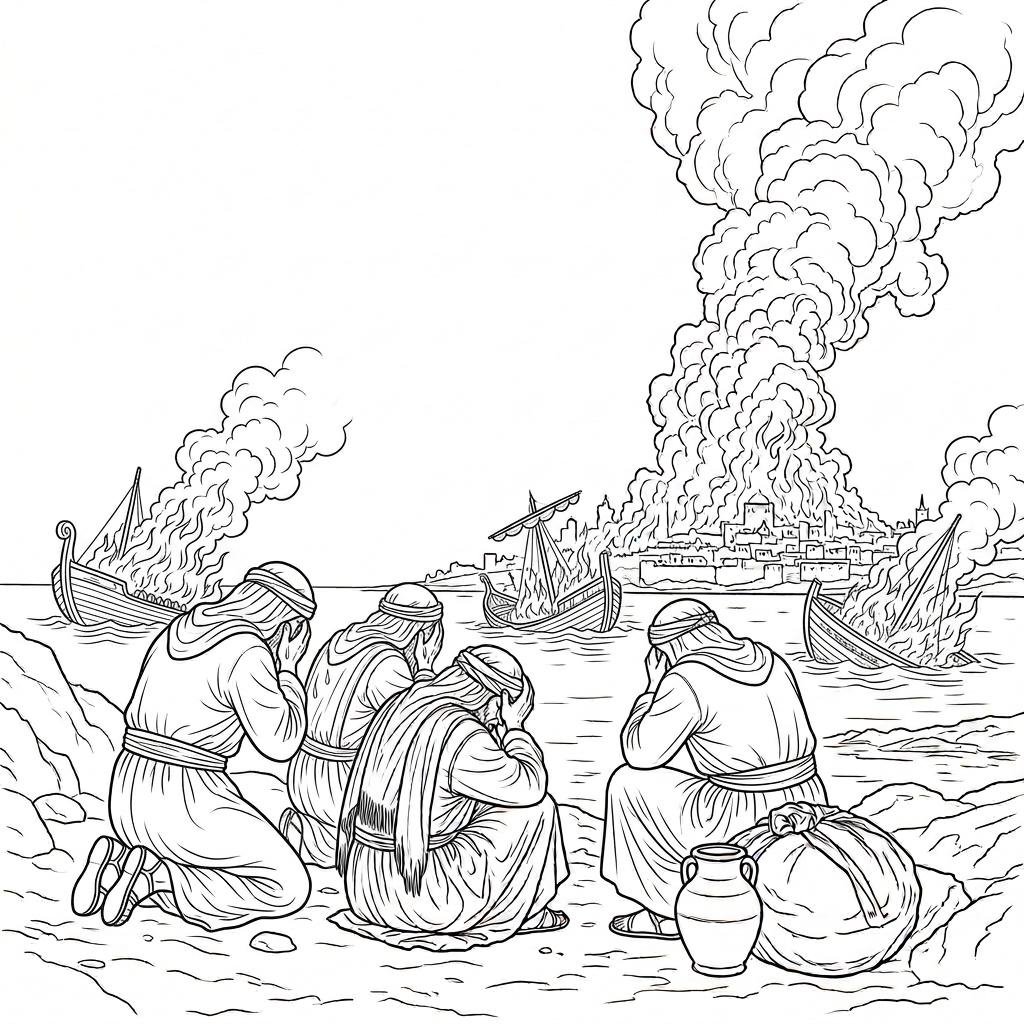
\includegraphics[
    width=0.9\textwidth,
    trim=0 0 0 0,
    clip]{images/rev_18_bablyon_burning.jpg}
    %\caption{}
    %\label{}
\end{figure}

The beast\index{beast} represents the power that opposes God. The ten horns\index{seven heads and ten horns} represent ten kings who unite with the beast. Babylon\index{Babylon}, portrayed as the great prostitute\index{great prostitute}, symbolizes a world system that seduces the nations through luxury, power, and economic gain. Bound together by shared interests, these powers surrender their authority to the beast and unite in opposition to the Lamb.

Yet their alliance does not endure. In the end, the ten horns\index{seven heads and ten horns} and the beast turn against the prostitute\index{great prostitute} herself. They strip her, devastate her, and consume her with fire. Their hostility reveals the instability of a kingdom built upon rebellion and self-interest. The forces opposed to God may form alliances for a season, but they cannot establish an everlasting order. God remains sovereign over history, even turning their mutual hatred against one another to accomplish His judgment.

For the early Church, Babylon\index{Babylon}'s downfall presented a choice with immediate and personal consequences. Rome\index{Rome} commanded formidable political power, controlled an extensive network of trade, and possessed extraordinary material wealth. Through imperial worship and other public expressions of loyalty, it also asserted its authority over the lives and consciences of its subjects.

When society demanded that Christians participate in idolatrous practices or express allegiance to the emperor and earthly powers in ways that contradicted their faith, they had to choose: Would they conform to the expectations of the surrounding world, or remain loyal to Jesus Christ?

\begin{ReaderQuestion}
God declares, “Come out of her, my people, so that you will not share in her sins.” What did this command mean for the early Church? What does it call the Church today to examine in its own life and witness?
\end{ReaderQuestion}

The contrast becomes even more striking when we compare Babylon\index{Babylon}, the prostitute\index{great prostitute} of Revelation 17 and 18, with the bride\index{bride of the Lamb} of the Lamb in Revelation 21. Table \ref{tab:babylon_bride} sets these two visions side by side.
{
\small
\renewcommand{\arraystretch}{1}
\begin{longtable}{>{\raggedright\arraybackslash}p{2.2cm}
                  >{\raggedright\arraybackslash}p{3.4cm}
                  >{\raggedright\arraybackslash}p{3.4cm}}
\caption{The Bride of the Holy City Is Beyond Compare}
\label{tab:babylon_bride} \\
\hline
Contrast & Babylon, the Prostitute (Chapter 18) & The Bride of the Holy City (Chapter 21) \\
\hline
\endfirsthead

\multicolumn{3}{l}{\small\itshape Table~\thetable\ (continued)} \\
\hline
Contrast & Babylon, the Prostitute (Chapter 18) & The Bride of the Holy City (Chapter 21) \\
\hline
\endhead

\hline
\endfoot

\hline
\endlastfoot

Passages &
17:1--6; 18:1--24 &
21:2, 9--10 \\

Symbolism &
A world system that seduces the nations. &
God's people, redeemed by the Lamb. \\

Outward appearance &
Clothed in purple and scarlet, adorned with gold, precious stones, and pearls. &
The city shines with the glory of God, radiant like a precious jewel (21:11). \\

Relationship with the nations &
The kings of the earth commit adultery with her. &
The kings of the earth bring their glory into the city (21:24--26). \\

Relationship with God &
Filled with abominations and stained with the blood of the saints. &
God's dwelling is among His people, and He lives with them (21:3). \\

Relationship with humanity &
Merchants grow rich through her extravagant luxury (18:3, 15--19). &
God freely gives the water of life to the thirsty (21:6, 17). \\

Tears and death &
The world mourns her destruction (18:9--19). &
God wipes away every tear; death, mourning, crying, and pain are no more (21:4). \\

Final destiny &
Destroyed and cast down (18:8--10, 21). &
Descends from heaven, to dwell with God and His people forever (21:2--3). \\

\end{longtable}
}

Babylon\index{Babylon} dazzles the world with splendor that cannot endure. The holy city\index{holy city} shines with a glory that comes from God and will never fade. Babylon enriches merchants, seduces rulers, and sheds the blood of the faithful; the New Jerusalem\index{New Jerusalem} welcomes God's redeemed\index{redemption} people into His presence. Babylon's admirers weep because their earthly treasures have vanished. In the holy city, God Himself wipes away every tear.

The contrast reaches beyond two cities or two women. It reveals two rival visions of glory. One seeks to ascend through wealth, domination, and self-exaltation, only to fall. The other receives its glory from God, belongs to the Lamb, and endures forever. The Christian life is shaped by the choice between them: to be captivated by what dazzles for a moment, or to remain faithful to the One whose kingdom has no end.

\begin{ReaderQuestion}
In what ways might believers today be drawn toward Babylon's values---wealth, success, power, pleasure, or human approval? How can we examine our hearts and recognize when these things are beginning to take God's place?
\end{ReaderQuestion}
